%\documentclass{beamer}
\documentclass[handout]{beamer}
\usepackage[spanish]{babel}
\usepackage[utf8]{inputenc}
\usepackage{graphicx}
\usepackage{multimedia}
\usepackage{animate}
\usepackage{tcolorbox}
\usepackage{amsmath}

\usebackgroundtemplate{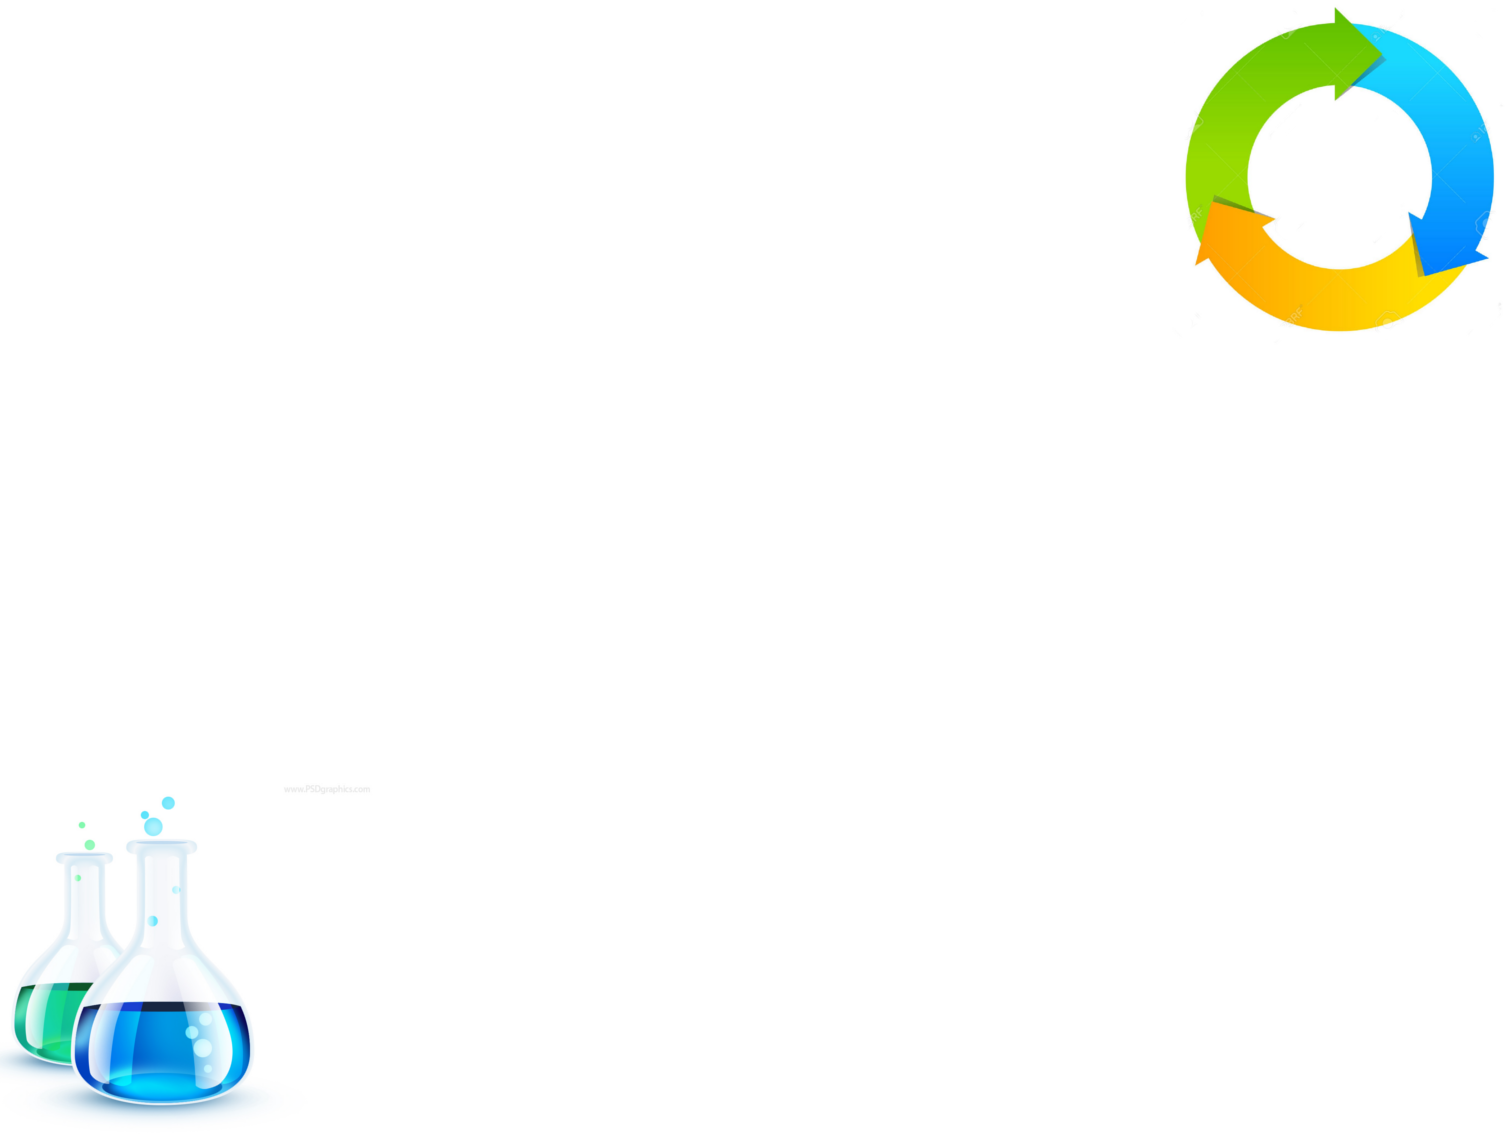
\includegraphics[width=\paperwidth]{sources/Background.png}}
\setbeamercolor{frametitle}{fg=black}
\usefonttheme{structuresmallcapsserif}
\setbeamertemplate{footline}[frame number]
\setbeamerfont{footnote}{size=\tiny}

\usepackage{default}

\usepackage[backend = bibtex, style = verbose, sorting = none, autocite = footnote]{biblatex}
\addbibresource{references.bib}

\definecolor{green}{RGB}{0, 150, 0}

\newcommand\blfootnote[1]
{%
	\begingroup
	\renewcommand\thefootnote{}\footnote{#1}%
	\addtocounter{footnote}{-1}%
	\endgroup
}
\newcommand{\fcite}[1]{\blfootnote{\cite{#1}}}
\newcommand{\kw}[1]{{\color{blue}#1}}
\newcommand{\cfigure}[2]
{
	\begin{figure}
		\centering
		\includegraphics[width = #2]{#1}
	\end{figure}
}

\begin{document}
{
	\begin{frame}
		\centering
		{
			\color{blue}
			\noindent\rule{6cm}{0.4pt}\\
			\textsc{\LARGE Ciclos catalíticos}\\
			\noindent\rule{6cm}{0.4pt}
		}
		\cfigure{sources/imagen_ciclo.png}{0.4\linewidth}
		\raggedleft
		{
			Juan Barbosa\\
			Universidad de los Andes
		}
	\end{frame}
}

\begin{frame}{Contenido}
	\begin{columns}
		\begin{column}{0.4\textwidth}
			\tableofcontents
		\end{column}
		\begin{column}{0.6\textwidth}
			\cfigure{sources/Market.jpg}{0.8\linewidth}
			\footnotesize Craqueo catalítico selectivo al propileno
		\end{column}
	\end{columns}
	\fcite{vogt2015fluid}
\end{frame}

\section{Introducción}

\subsection{Historia}
\begin{frame}{Historia}
	\begin{itemize}
		\item Las trazas más antiguas de vino son del 6000 a.C.
		\item La existencia de levaduras permite fermentar los frutos.
	\end{itemize}
	\begin{columns}
		\begin{column}{0.4\textwidth}
			\cfigure{sources/wine.jpg}{\textwidth}
		\end{column}
		\begin{column}{0.6\textwidth}
			\cfigure{sources/sugar.png}{\linewidth}
		\end{column}
	\end{columns}
	\fcite{mcgovern2003origins}
\end{frame}

\begin{frame}{Historia}
	\begin{itemize}
		\item No fue hasta 1887 que los mecanismos de reacción empezaron a ser estudiados.
	\end{itemize}
	\begin{columns}
		\begin{column}{0.2\textwidth}
			\cfigure{sources/Henry_Armstrong.jpg}{\textwidth}
			Henry Armstrong
		\end{column}
		\begin{column}{0.6\textwidth}
			\cfigure{sources/SE.png}{\linewidth}
			Sustitución electrofílica aromática
		\end{column}
	\end{columns}
	\fcite{armstrong1887xxviii}
\end{frame}

\begin{frame}{Historia}
	\begin{itemize}
		\item En el siglo XX emerge la catálisis.
	\end{itemize}
	\begin{columns}
		\begin{column}{0.2\textwidth}
			\cfigure{sources/sabatier.jpg}{\textwidth}
			Paul Sabatier
		\end{column}
		\begin{column}{0.3\textwidth}
			\cfigure{sources/grignard.jpg}{0.7\linewidth}
			Victor Grignard
		\end{column}
		\begin{column}{0.5\textwidth}
			"Por el método de hidrogenación de compuestos orgánicos en presencia de metales finamente desintegrados"
		\end{column}
	\end{columns}
	\fcite{astruc2007organometallic}
	\fcite{kagan2012victor}
\end{frame}

\begin{frame}{Historia}
	\begin{itemize}
		\item Realiza los primeros estudios detallados de la cinética del mecanismo de reacción.
	\end{itemize}
	\begin{columns}
		\begin{column}{0.2\textwidth}
			\cfigure{sources/wilkinson1.png}{\textwidth}
			Sir Geoffrey Wilkinson
		\end{column}
		\begin{column}{0.5\textwidth}
			"Por el trabajo, realizado de manera independiente, en la química organometálica"
		\end{column}
	\end{columns}
	\fcite{astruc2007organometallic}
	\fcite{kagan2012victor}
\end{frame}

\begin{frame}{Introducci\'on}
	\begin{columns}
		\begin{column}{0.5\textwidth}
			\begin{itemize}
				\item \color{blue} Un catalizador:
				\begin{itemize}
					\item Permite que una reacci\'on ocurra m\'as r\'apidamente.
					\item Cantidades estequeom\'etricas de $10^{-6}-10^{-1}$.
					\item Se recupera al final de la reacci\'on.
					\item No influencia la termodin\'amica de la reacci\'on.
					\item Es caracterizado por su \kw{TOF}, y \kw{TON}.
				\end{itemize}
			\end{itemize}
		\end{column}
		\begin{column}{0.6\textwidth}
			\begin{itemize}
				\item \color{blue} Un ciclo catal\'itico:
				\begin{itemize}
					\item Es un mecanismo de reacción en varios pasos que involucra a un catalizador.
					\item Es el método principal para describir el papel de los catalizadores.
					\item Suele ser escrito como una secuencia de reacciones en la forma de un anillo.
				\end{itemize}
			\end{itemize}
		\end{column}
	\end{columns}
	\fcite{astruc2007organometallic}
\end{frame}

\begin{frame}{Introducci\'on}
	\begin{itemize}
		\item \kw{TON:} Turn Over Number
		\begin{equation}
			TON = \dfrac{\text{\# moles de producto}}{\text{\# moles de catalizador}}
		\end{equation}
		\item \kw{TOF:} Turn Over Frequency
		\begin{equation}
			TOF = \dfrac{\text{\# moles de producto}}{\text{tiempo}\times\text{\# moles de catalizador}} = \dfrac{TON}{\text{tiempo}}
		\end{equation}
	\end{itemize}
	El \kw{TON} y \kw{TOF} son medidas de actividad.
	\begin{itemize}
		\footnotesize
		\item En catálisis homogénea es la
		cantidad de materia en solución.
		\item En catálisis heterogénea depende de la superficie.
	\end{itemize}
	\fcite{astruc2007organometallic}
\end{frame}

\subsection{Tipos de ciclos}
\begin{frame}{Tipos de ciclos}
    \begin{columns}
        \begin{column}{0.5\textwidth}
            \begin{itemize}
                \item Homogéneos
                \begin{itemize}
                	\item Sitios de coordinaci\'on vacantes.
                	\item Metales con 16 o 14 $e^-$.
                	\item Esp\'ecies que se alternan entre 16 y 18 $e^-$.
                \end{itemize}
                \item Enzim\'aticos
                \begin{itemize}
                	\item An\'alogos a los homog\'eneos, pero considerablemente m\'as complejos.
                	\item Cuentan con la mayor eficiencia.
            	\end{itemize}
            \end{itemize}
        \end{column}
        \begin{column}{0.5\textwidth}
            \begin{itemize}
                \item Heterogéneos
            	\begin{itemize}
            		\item Procesos de adsorción y desorción.
            		\item Difíciles de estudiar.
            	\end{itemize}
            \end{itemize}
        \end{column}
    \end{columns}
	\fcite{astruc2007organometallic}
	\fcite{jens2014fundamental}
\end{frame}

\section{Aplicaciones}
\begin{frame}{Aplicaciones}
    \begin{columns}
        \begin{column}{0.5\textwidth}
            \begin{itemize}
                \item Qu\'imica atmosf\'erica
                \cfigure{sources/clouds.jpg}{0.8\linewidth}
                \item Qu\'imica org\'anica
                \cfigure{sources/hydrogenation.png}{0.8\linewidth}
%                \item Industria
            \end{itemize}
        \end{column}
        \begin{column}{0.5\textwidth}
            \begin{itemize}
                \item Bioqu\'imica
                \cfigure{sources/enzymatic.jpg}{0.8\linewidth}
                \item Industria
                \cfigure{sources/industry.jpg}{\linewidth}
%                \item Termodin\'amica
%                \cfigure{sources/thermo.jpg}{0.8\linewidth}
            \end{itemize}
        \end{column}
    \end{columns}
\end{frame}

\subsection{Química atmosférica}
\begin{frame}{Qu\'imica atmosf\'erica}
	\begin{columns}
		\begin{column}{0.5\textwidth}
			\movie[height = 0.6\textwidth, width = \textwidth, poster, showcontrols]{}{sources/o3split.mp4}
		\end{column}
		\begin{column}{0.5\linewidth}
			\begin{figure}[h]
				\centering
				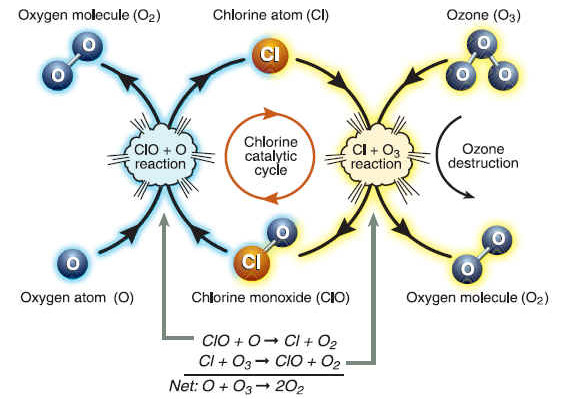
\includegraphics[scale = 0.125]{sources/ozone.jpg}
			\end{figure}
		\end{column}
	\end{columns}
\end{frame}

\begin{frame}{Qu\'imica atmosf\'erica}
	\cfigure{sources/stratospheric_chlorine.png}{0.7\linewidth}
	\fcite{ravishankara2009nitrous}
\end{frame}

\subsection{Bioqu\'imica}
\begin{frame}{Bioqu\'imica}
	\begin{figure}[h]
		\centering
		\movie[height = 0.3\textwidth, width = 0.5\textwidth, poster, showcontrols]{}{sources/enzyme.mp4}
	\end{figure}
	\cfigure{sources/enzymeCycle.png}{0.7\linewidth}
\end{frame}

\begin{frame}{Bioqu\'imica}
	\begin{itemize}
		\item Reacción monooxigenasa:
		\begin{equation}
			RH + O_2 + 2H^+ + 2e^- -> ROH + H_2O 
		\end{equation}
	\end{itemize}
	\begin{columns}
		\begin{column}{0.5\textwidth}
			\begin{enumerate}
				\item Unión del sustrato
				\item Primera reducci\'on
				\item Uni\'on del ox\'igeno
				\item Segunda reducci\'on
				\item Liberaci\'on de agua
				\item Migraci\'on de H
				\item Liberaci\'on del producto
			\end{enumerate}
		\end{column}
		\begin{column}{0.5\textwidth}
			\cfigure{sources/P450.png}{0.9\linewidth}
		\end{column}
	\end{columns}
	\fcite{de2005cytochrome}
%	es decir, la inserción de un átomo de oxígeno proveniente de oxígeno molecular (O$_2$) en un sustrato orgánico (RH) a la vez que el otro átomo de oxígeno es reducido a agua
\end{frame}


\subsection{Química org\'anica}
\begin{frame}{Qu\'imica org\'anica}
	Hidrogenaci\'on de Wilkinson
	\begin{columns}
		\begin{column}{0.5\textwidth}
			\cfigure{sources/wilkinson.png}{\textwidth}
		\end{column}
		\begin{column}{0.5\textwidth}
			\begin{enumerate}
				\item Obtención de la espécie activa
				\item Adici\'on oxidativa del H$_2$
				\item Complejo $\pi$ con la olefina
				\item Migraci\'on de H
				\item Eliminaci\'on reductiva
			\end{enumerate}
		\end{column}
	\end{columns}
	\fcite{bhaduri2014homogeneous}
%The mechanism of this reaction involves the initial dissociation of one or two triphenylphosphine ligands to give 14- or 12-electron complexes, respectively, followed by oxidative addition of H2 to the metal. Subsequent π-complexation of alkene, migratory insertion (intramolecular hydride transfer or olefin insertion), and reductive elimination complete the formation of the alkane product,
\end{frame}

%\subsection{Termodin\'amica}
%\begin{frame}{Termodin\'amica}
%\begin{columns}
%	\begin{column}{0.5\textwidth}
%	\end{column}
%	\begin{column}{0.5\textwidth}
%	\end{column}
%\end{columns}
%\end{frame}

\subsection{Industria}
\begin{frame}{Industria}
	Hidrogenaci\'on de alquenos
	
	\cfigure{sources/hydrogenation.png}{0.8\linewidth}
	\fcite{van2014challenges}
\end{frame}

\begin{frame}{Industria}
	Proceso Haber-Bosch
	\begin{columns}
		\begin{column}{0.6\textwidth}
			\cfigure{sources/haberBosch.jpg}{\linewidth}
		\end{column}
		\begin{column}{0.5\textwidth}
			\begin{itemize}
				\item No se conoce con certeza el ciclo catal\'itico.
				\item Se cree que los siguientes pasos ocurren.
				\begin{enumerate}
					\item Adsorci\'on de los gases.
					\item Disociaci\'on de las mol\'eculas.
					\item Formaci\'on de NH, NH$_2$ y NH$_3$.
					\item Desorci\'on.
				\end{enumerate}
			\end{itemize}
		\end{column}
	\end{columns}
	\fcite{van2014challenges}
\end{frame}

\begin{frame}
	\centering
	\Huge
	Gracias
\end{frame}


\end{document}